\section{Технологический раздел}

В данном разделе обосновывается выбор средств программной реализации разработанного метода оценки кредитоспособности физических лиц, описывается структура программного обеспечения, реализующего алгоритм градиентного бустинга деревьев решений, а также приводится описание формата входных и выходных данных и принципов взаимодействия компонентов системы.

\subsection{Обоснование выбора технологий}

Для реализации разработанного метода оценки кредитоспособности физических лиц были выбраны два основных инструмента: язык программирования Python и язык C\#.

Python используется для реализации алгоритмов машинного обучения, обработки данных и построения модели кредитного скоринга, тогда как язык C\# применяется для разработки пользовательского интерфейса, обеспечивающего взаимодействие пользователя с системой.

Язык Python выбран благодаря следующим преимуществам:
\begin{itemize}
  \item высокая производительность при работе с числовыми данными и большими объемами информации;
  \item широкое распространение в задачах анализа данных, финансового моделирования и кредитного скоринга;
  \item наличие инструментов для визуализации и интерпретации результатов работы моделей;
  \item поддержка современных алгоритмов машинного обучения, включая градиентный бустинг.
\end{itemize}

Для разработки пользовательского интерфейса был выбран язык C\# с использованием технологии Windows Forms. Данный выбор обусловлен следующими причинами:

\begin{itemize}
  \item возможность быстрого создания настольных приложений с графическим интерфейсом;
  \item интеграция с операционной системой Windows;
  \item возможность взаимодействия с внешними процессами, включая запуск Python-скриптов.
\end{itemize}

В рамках реализации программного комплекса были использованы следующие основные библиотеки и инструменты:

\begin{itemize}
  \item \textbf{pandas} -- для обработки и анализа табличных данных;
  \item \textbf{numpy} -- для выполнения численных операций;
  \item \textbf{scikit-learn} -- для подготовки данных, оценки качества модели и расчета метрик;
  \item \textbf{LightGBM} -- для реализации алгоритма градиентного бустинга деревьев решений;
  \item \textbf{matplotlib} -- для визуализации результатов, включая ROC- и PR-кривые;
  \item \textbf{joblib} -- для сохранения и загрузки обученной модели;
  \item \textbf{C\# (Windows Forms)} -- для разработки пользовательского интерфейса системы.
\end{itemize}

Выбор библиотеки LightGBM обусловлен ее высокой скоростью обучения, эффективной работой с большими объемами данных и встроенной поддержкой обработки пропущенных значений. Кроме того, данный алгоритм хорошо подходит для решения задач кредитного скоринга, поскольку способен выявлять сложные нелинейные зависимости между признаками и обеспечивает высокое качество классификации.

%-------------------------

\subsection{Основные программные модули системы}

Разработанное программное обеспечение включает несколько взаимосвязанных модулей, реализующих подготовку данных, обучение модели машинного обучения и оценку кредитоспособности заемщика.

Структура программного комплекса и взаимодействие его основных компонентов представлены на рисунке \ref{fig:architecture_scheme}.

\FloatBarrier
\begin{figure}[ht!]
  \begin{center}
    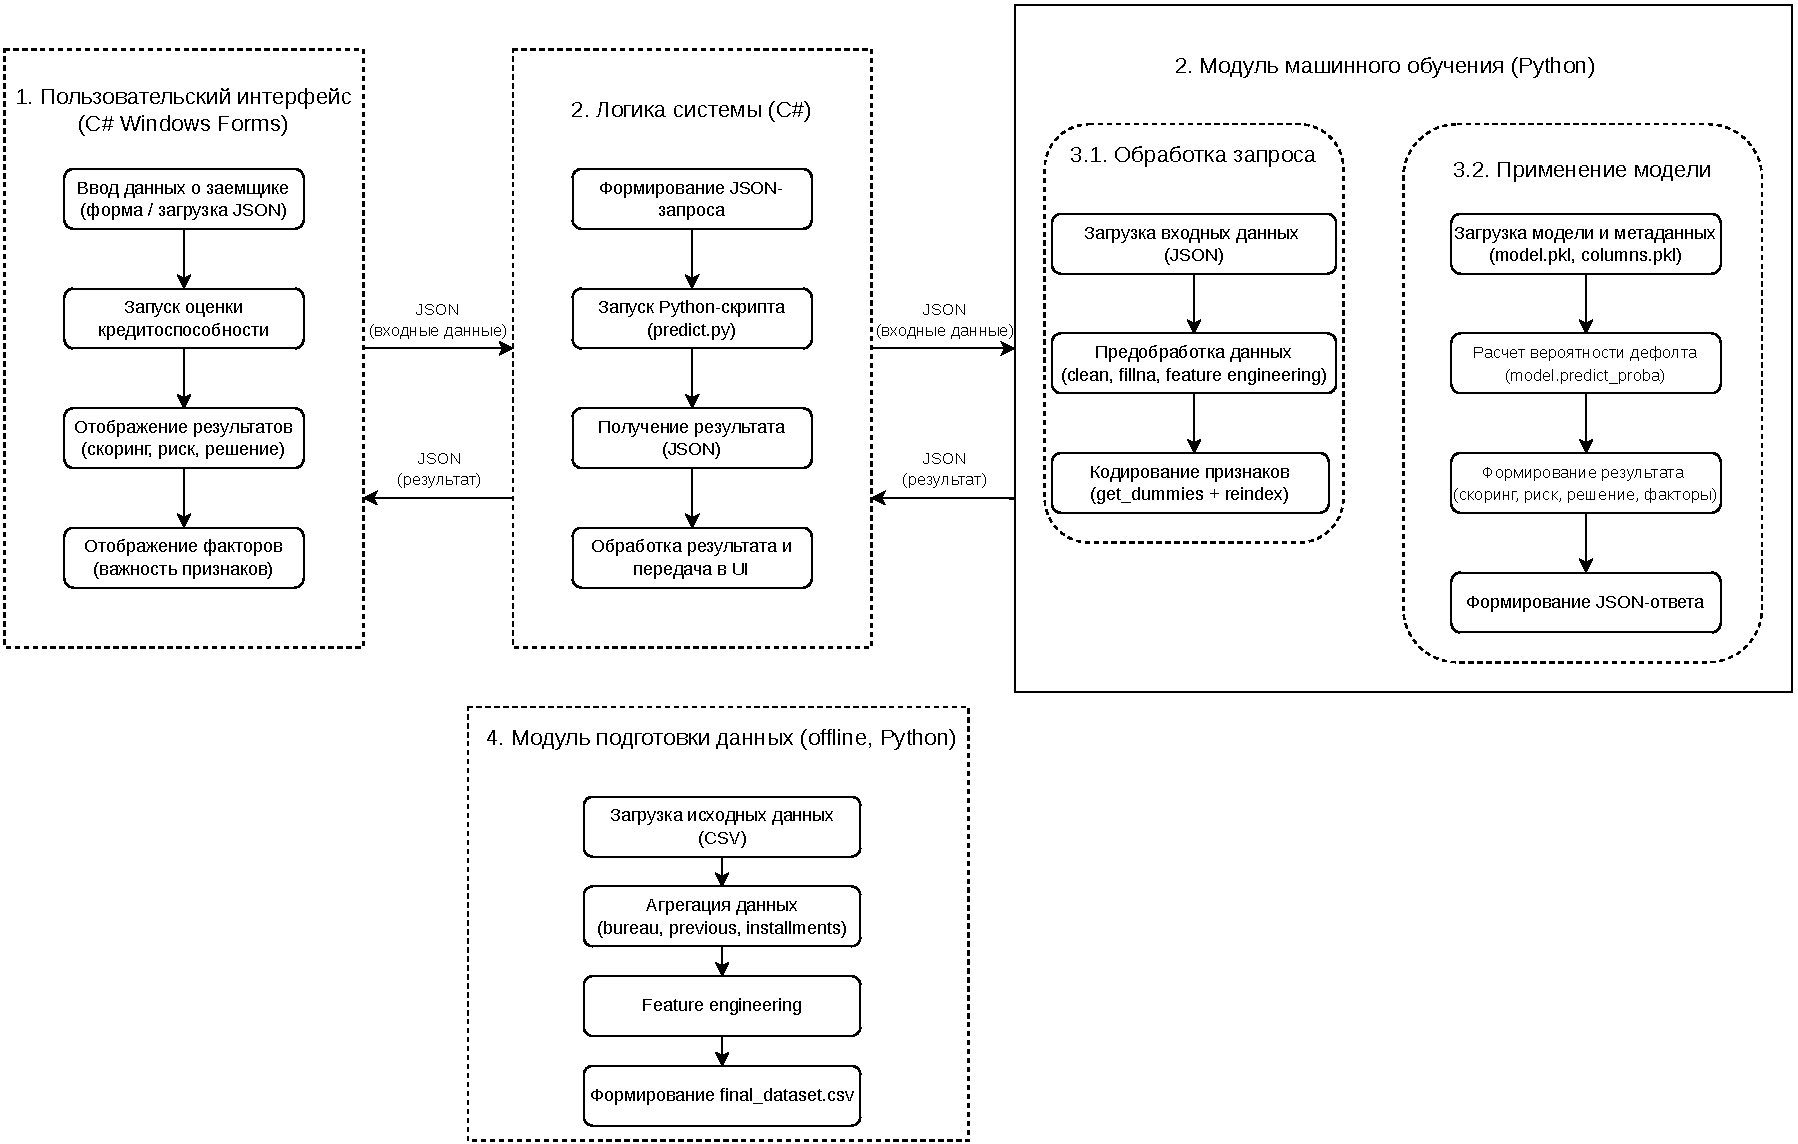
\includegraphics[width=\linewidth, height=0.9\textheight, keepaspectratio]{inc/pdf/Структурная схема взаимодействия компонентов системы.drawio.pdf}
  \end{center}
  \captionsetup{justification=centering}
  \caption{Структурная схема взаимодействия компонентов системы оценки кредитоспособности}
  \label{fig:architecture_scheme}
\end{figure}
\FloatBarrier

На рисунке представлена структура разработанной системы, а также схема взаимодействия между ее основными программными модулями. Система включает этапы подготовки данных, обучения модели, формирования прогнозов и отображения результатов пользователю.

Первым этапом работы системы является формирование набора данных для обучения модели. Для этого используется модуль предварительной обработки данных, реализованный на языке Python. Модуль выполняет загрузку исходных CSV-файлов, содержащих информацию о заемщиках, кредитной истории, предыдущих заявках и платежах по кредитам.

После загрузки выполняется агрегация данных по каждому заемщику, обработка пропущенных значений и формирование дополнительных признаков. В процессе feature engineering рассчитываются производные показатели, характеризующие долговую нагрузку клиента, уровень просрочек, соотношение кредита к доходу, кредитную активность и другие параметры. Итоговый набор данных сохраняется в файл \texttt{final\_dataset.csv} и используется для последующего обучения модели.

Обучение модели реализовано в отдельном модуле на языке Python с использованием библиотеки LightGBM. Модуль выполняет загрузку подготовленного набора данных, разделение выборки на обучающую и тестовую части, кодирование категориальных признаков методом one-hot encoding и обучение модели градиентного бустинга деревьев решений.

В процессе обучения модели учитывалась проблема дисбаланса классов, характерная для задач кредитного скоринга, при которой количество заемщиков с дефолтом существенно меньше количества надежных клиентов. Для компенсации данного дисбаланса использовался параметр \texttt{scale\_pos\_weight}, позволяющий повысить чувствительность модели к выявлению рискованных заемщиков. Подбор оптимальных гиперпараметров осуществлялся с применением методов RandomizedSearchCV и GridSearchCV.

После завершения обучения выполняется расчет основных метрик качества модели, включая ROC-AUC, Precision, Recall и F1-score. Обученная модель сохраняется в файл \texttt{model.pkl}, а список признаков — в файл \texttt{columns.pkl}.

Для оценки кредитоспособности заемщика используется отдельный модуль предсказания. Данный модуль загружает обученную модель, принимает входные данные в формате JSON, выполняет предобработку и расчет вероятности дефолта с использованием функции \texttt{predict\_proba}.

На основе полученной вероятности формируется скоринговый балл, уровень риска заемщика и рекомендации по принятию кредитного решения. Дополнительно реализован механизм интерпретации результатов с использованием библиотеки SHAP, позволяющий определить признаки, оказавшие наибольшее влияние на итоговое решение модели.

Пользовательский интерфейс системы реализован на платформе Windows Forms с использованием языка C\#. Интерфейс обеспечивает ввод параметров заемщика, загрузку JSON-файлов и отображение результатов скоринга. Взаимодействие между C\#-приложением и Python-модулем реализовано посредством запуска Python-скрипта через класс \texttt{ProcessStartInfo} с последующим чтением результата из стандартного потока вывода.

Полные листинги основных программных модулей приведены в приложении А.

%--------------------------
\subsection{Формат входных и выходных данных}

Входные данные системы представляют собой информацию о заемщике, представленную в формате JSON.

Структура входных данных включает:

\begin{itemize}
  \item финансовые характеристики (доход, сумма кредита, размер платежей);
  \item социально-демографические данные;
  \item параметры кредитной истории;
  \item агрегированные показатели поведения заемщика.
\end{itemize}

Выходные данные системы также формируются в формате JSON и содержат:

\begin{itemize}
  \item вероятность дефолта;
  \item скоринговый балл;
  \item уровень кредитного риска;
  \item решение о выдаче кредита;
  \item факторы, влияющие на решение модели.
\end{itemize}

%--------------------------

\subsection{Тестирование программного обеспечения}

Тестирование программы выполнено на реальных данных открытого набора Home Credit Default Risk, размещенного в открытом доступе на платформе Kaggle, а также на синтетически сформированных наборах данных, предназначенных для проверки различных сценариев функционирования программного комплекса \cite{KaggleHomeCreditDefaultRisk}.

Целью тестирования являлась проверка корректности работы программного комплекса и итоговой модели оценки кредитоспособности. Проверялись ввод данных заемщика, формирование входного JSON-файла, запуск Python-модуля предсказания, получение результата скоринга и отображение результата в пользовательском интерфейсе.
\newpage
В ходе тестирования проверялись следующие сценарии:
\begin{itemize}
  \item ручной ввод данных заемщика через формы приложения;
  \item формирование JSON-структуры на основе введенных данных;
  \item загрузка данных заемщика из JSON-файла;
  \item получение результата работы модели в формате JSON;
  \item отображение вероятности дефолта, скорингового балла и уровня риска;
  \item отображение факторов риска и рекомендаций;
  \item обработка ошибок при отсутствии файла или некорректных входных данных.
\end{itemize}

Для проверки качества итоговой модели исходный набор данных был разделен на обучающую и тестовую выборки в соотношении 80\% и 20\%. Тестовая выборка не использовалась при обучении модели, что позволило оценить качество работы метода на новых данных.

По результатам тестирования обученной модели были получены значения основных метрик качества, представленные в таблице~\ref{tab:metrics}.

\begin{table}[ht!]
  \centering
  \caption{Метрики качества итоговой модели}
  \label{tab:metrics}
  \begin{tabular}{|c|c|}
    \hline
    Метрика   & Значение \\
    \hline
    Accuracy  & 0.48     \\
    ROC-AUC   & 0.777    \\
    Precision & 0.12     \\
    Recall    & 0.89     \\
    F1-score  & 0.22     \\
    \hline
  \end{tabular}
\end{table}

Полученные значения показывают, что модель обладает высокой полнотой выявления дефолтных заемщиков. Значение Recall составило 0.89, что означает способность модели обнаруживать значительную часть заемщиков с высоким риском дефолта. При этом значение Precision составило 0.12, что указывает на наличие большого количества ложноположительных решений.

Такая особенность является допустимой для рассматриваемой задачи, поскольку в кредитном скоринге пропуск заемщика с высоким риском дефолта может привести к финансовым потерям. Поэтому в рамках работы приоритет был отдан повышению полноты выявления дефолтных заемщиков.

Дополнительно была построена матрица ошибок, представленная в таблице~\ref{tab:confusion_matrix}.

\begin{table}[ht!]
  \centering
  \caption{Матрица ошибок итоговой модели}
  \label{tab:confusion_matrix}
  \begin{tabular}{|c|c|c|}
    \hline
                 & Предсказано 0 & Предсказано 1 \\
    \hline
    Фактически 0 & 24972         & 31566         \\
    \hline
    Фактически 1 & 561           & 4404          \\
    \hline
  \end{tabular}
\end{table}

Из матрицы ошибок видно, что модель правильно выявила 4404 заемщика с дефолтом. Количество пропущенных дефолтных заемщиков составило 561. При этом 31566 надежных заемщиков были ошибочно отнесены к группе риска. Такой результат объясняется выбранным порогом классификации, равным 0.3, который был установлен для повышения полноты выявления дефолтов.

Для оценки влияния порога классификации был проведен дополнительный анализ количества ошибок при различных значениях порога. Результаты представлены в таблице~\ref{tab:threshold}.

\begin{table}[ht!]
  \centering
  \caption{Зависимость ошибок от порога классификации}
  \label{tab:threshold}
  \begin{tabular}{|c|c|c|}
    \hline
    Порог & FN   & FP    \\
    \hline
    0.30  & 561  & 31566 \\
    0.50  & 1563 & 15323 \\
    0.70  & 3112 & 4462  \\
    \hline
  \end{tabular}
\end{table}

Анализ показал, что увеличение порога классификации снижает количество ложноположительных решений, однако одновременно увеличивает число пропущенных дефолтных заемщиков. Поэтому для итоговой модели был выбран порог 0.3. Такой порог позволяет уменьшить количество пропущенных дефолтов, что соответствует специфике задачи кредитного скоринга.

На рисунке~\ref{fig:roc_curve} представлена ROC-кривая итоговой модели.

\FloatBarrier
\begin{figure}[ht!]
  \begin{center}
    
\includegraphics[width=0.65\linewidth]{inc/png/roc_curve.png}
  \end{center}
  \captionsetup{justification=centering}
  \caption{ROC-кривая итоговой модели}
  \label{fig:roc_curve}
\end{figure}
\FloatBarrier

ROC-кривая показывает, что модель обладает способностью разделять заемщиков по уровню кредитного риска. Значение ROC-AUC, равное 0.777, подтверждает, что модель выполняет ранжирование заемщиков лучше случайного классификатора.

На рисунке~\ref{fig:pr_curve} представлена Precision-Recall кривая итоговой модели.

\FloatBarrier
\begin{figure}[ht!]
  \begin{center}
    
\includegraphics[width=0.65\linewidth]{inc/png/pr_curve.png}
  \end{center}
  \captionsetup{justification=centering}
  \caption{Precision-Recall кривая итоговой модели}
  \label{fig:pr_curve}
\end{figure}
\FloatBarrier

Precision-Recall кривая использовалась для оценки качества выявления положительного класса при наличии дисбаланса данных. Она показывает соотношение точности и полноты при изменении порога классификации.

Для проверки работы ручного ввода были подготовлены синтетические тестовые наборы данных, соответствующие различным профилям заемщиков: заемщик с низким уровнем риска, заемщик со средней кредитной нагрузкой, заемщик с высоким уровнем риска, пенсионер, а также заемщик с большим количеством просрочек и отказов. Использование таких наборов позволило проверить корректность заполнения всех полей формы и передачу данных в модель.

Результаты проведенного функционального тестирования разработанного программного обеспечения приведены в таблице~\ref{tab:software_testing}.

\begin{table}[ht!]
  \centering
  \caption{Результаты функционального тестирования}
  \label{tab:software_testing}
  \begin{tabular}{|p{0.38\linewidth}|p{0.42\linewidth}|p{0.12\linewidth}|}
    \hline
    Проверяемый сценарий              & Ожидаемый результат                                                                                & Результат \\
    \hline
    Ручной ввод данных заемщика       & Данные принимаются системой и проходят проверку заполнения                                         & Успешно   \\
    \hline
    Формирование JSON по данным формы & Создается JSON-структура, соответствующая формату входных данных модели                            & Успешно   \\
    \hline
    Загрузка данных из JSON-файла     & Файл считывается, данные передаются в модуль предсказания                                          & Успешно   \\
    \hline
    Запуск Python-скрипта из C\#      & Python-модуль запускается из приложения и получает путь к входному файлу                           & Успешно   \\
    \hline
    Получение результата скоринга     & Приложение получает JSON с вероятностью дефолта, баллом и уровнем риска                            & Успешно   \\
    \hline
    Отображение результата            & На форме отображаются вероятность дефолта, скоринговый балл, уровень риска, факторы и рекомендации & Успешно   \\
    \hline
    Обработка некорректных данных     & Пользователю выводится сообщение об ошибке без аварийного завершения программы                     & Успешно   \\
    \hline
  \end{tabular}
\end{table}

Примеры работы пользовательского интерфейса при выполнении тестирования представлены на рисунках~\ref{fig:test_client_form}--\ref{fig:test_result_form}.
\newpage
На рисунке~\ref{fig:test_client_form} показана форма ручного ввода данных заемщика.

\FloatBarrier
\begin{figure}[ht!]
  \centering
  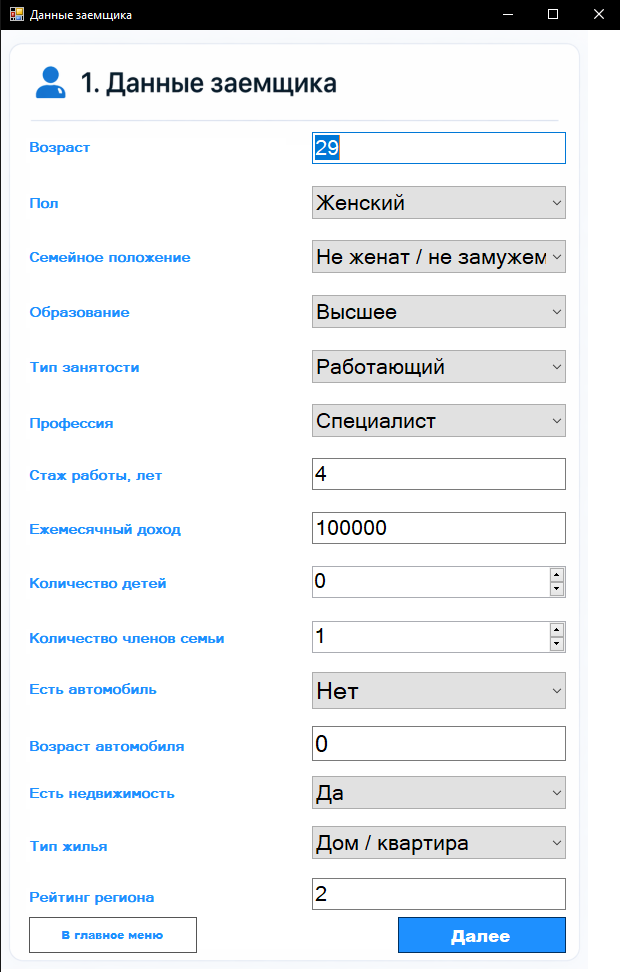
\includegraphics[width=0.65\linewidth]{inc/png/test_client_form.png}
  \caption{Форма ручного ввода данных заемщика}
  \label{fig:test_client_form}
\end{figure}
\FloatBarrier
\newpage
На рисунке~\ref{fig:test_credit_form} представлена форма ввода параметров кредита.

\FloatBarrier
\begin{figure}[ht!]
  \centering
  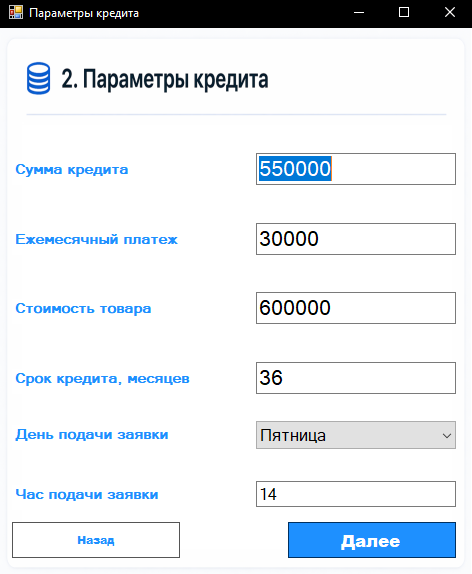
\includegraphics[width=0.65\linewidth]{inc/png/test_credit_form.png}
  \caption{Форма ввода параметров кредита}
  \label{fig:test_credit_form}
\end{figure}
\FloatBarrier
\newpage
На рисунке~\ref{fig:test_history_form} представлена форма ввода сведений о кредитной истории и платежном поведении заемщика.

\FloatBarrier
\begin{figure}[ht!]
  \centering
  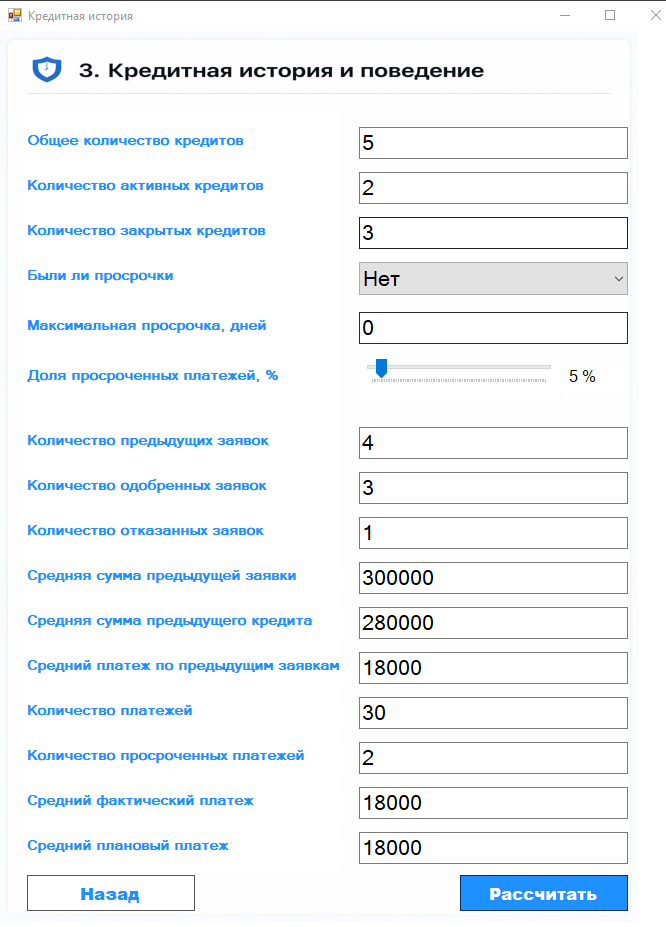
\includegraphics[width=0.7\linewidth]{inc/png/test_history_form.png}
  \caption{Форма ввода сведений о кредитной истории заемщика}
  \label{fig:test_history_form}
\end{figure}
\FloatBarrier
\newpage
На рисунке~\ref{fig:test_result_form} показан результат скоринга, полученный после обработки введенных данных, а также JSON-структура, сформированная программой при ручном вводе и переданная в модуль предсказания.

\FloatBarrier
\begin{figure}[ht!]
  \centering
  
\includegraphics[width=0.85\linewidth]{inc/png/test_result_form.png}
  \caption{Форма отображения результата скоринга и просмотр сформированного JSON}
  \label{fig:test_result_form}
\end{figure}
\FloatBarrier

Таким образом, тестирование подтвердило корректность работы основных компонентов программного комплекса. Итоговая модель корректно рассчитывает вероятность дефолта, а приложение обеспечивает ввод данных, формирование JSON, запуск Python-модуля, получение результата и отображение скоринговой оценки пользователю.

%--------------------------
\subsection*{Выводы}

В данном разделе были рассмотрены вопросы программной реализации разработанного метода оценки кредитоспособности физических лиц.

Обоснован выбор языка программирования Python для реализации модулей обработки данных, обучения и предсказания, а также языка C\# и технологии Windows Forms для разработки пользовательского интерфейса.

Описана структура программного комплекса, включающая модуль формирования набора данных, модуль обучения модели, модуль предсказания кредитоспособности и пользовательский интерфейс.

Определены форматы входных и выходных данных, используемые при взаимодействии между приложением и Python-модулем предсказания.

Проведено тестирование программного обеспечения на тестовой выборке и синтетических наборах данных. Результаты тестирования подтвердили корректность формирования входного JSON, запуска Python-модуля, получения результата скоринга и отображения итоговой оценки пользователю.